\documentclass[12pt]{article}
\usepackage{graphicx}%Package um Grafiken einzufügen
\graphicspath{ {assets/} }
\usepackage[ngerman]{babel}%Sprache Deutsch einstellen
\usepackage[headheight=15pt, a4paper, left=4cm, top=2cm, bottom=2cm, right=2cm]{geometry}
\usepackage[]{fontspec}
\setmonofont{CascadiaCode.ttf}[Scale=0.88]
\usepackage[]{fancyhdr}
\pagestyle{fancy}
%\setlength{\headheight}{16pt}
\lhead{\leftmark}
\rhead{Phillip Bronzel} 

\usepackage[style=authoryear, backend=biber]{biblatex}
\addbibresource{references.bib}
\usepackage{csquotes}

\usepackage{eso-pic}
\newcommand\BackgroundPic{
    \put(0,0){
    \parbox[b][\paperheight]{\paperwidth}{
    \vfill
    \centering
    
\includegraphics[width=\paperwidth,height=\paperheight]{assets/titlebackground.pdf}
    \vfill
    }}}

\usepackage{chronology}

\usepackage{subfig}

\usepackage{pgfplots}

\usepackage[onehalfspacing]{setspace}

\usepackage[bottom]{footmisc}

\usepackage{wrapfig}

\usepackage{xcolor}

\usepackage{svg}

\usepackage{float}

\usepackage{minted}
\usemintedstyle{pastie}
\renewcommand\listoflistingscaption{Quellcodeverzeichnis}

\usepackage{amsmath}

\usepackage{tikz}
\usetikzlibrary{matrix,calc,arrows.meta,bending}

\usepackage{ifthen}

\setcounter{secnumdepth}{3} \setcounter{tocdepth}{4}

\title{Machine Learning in Smartphone Apps}
\date{Phillip Bronzel \today}
\author{ASGSG Informatik, 2020/2021}

\begin{document}
\AddToShipoutPicture*{\BackgroundPic}
\maketitle
\pagenumbering{gobble}
\begin{center}
    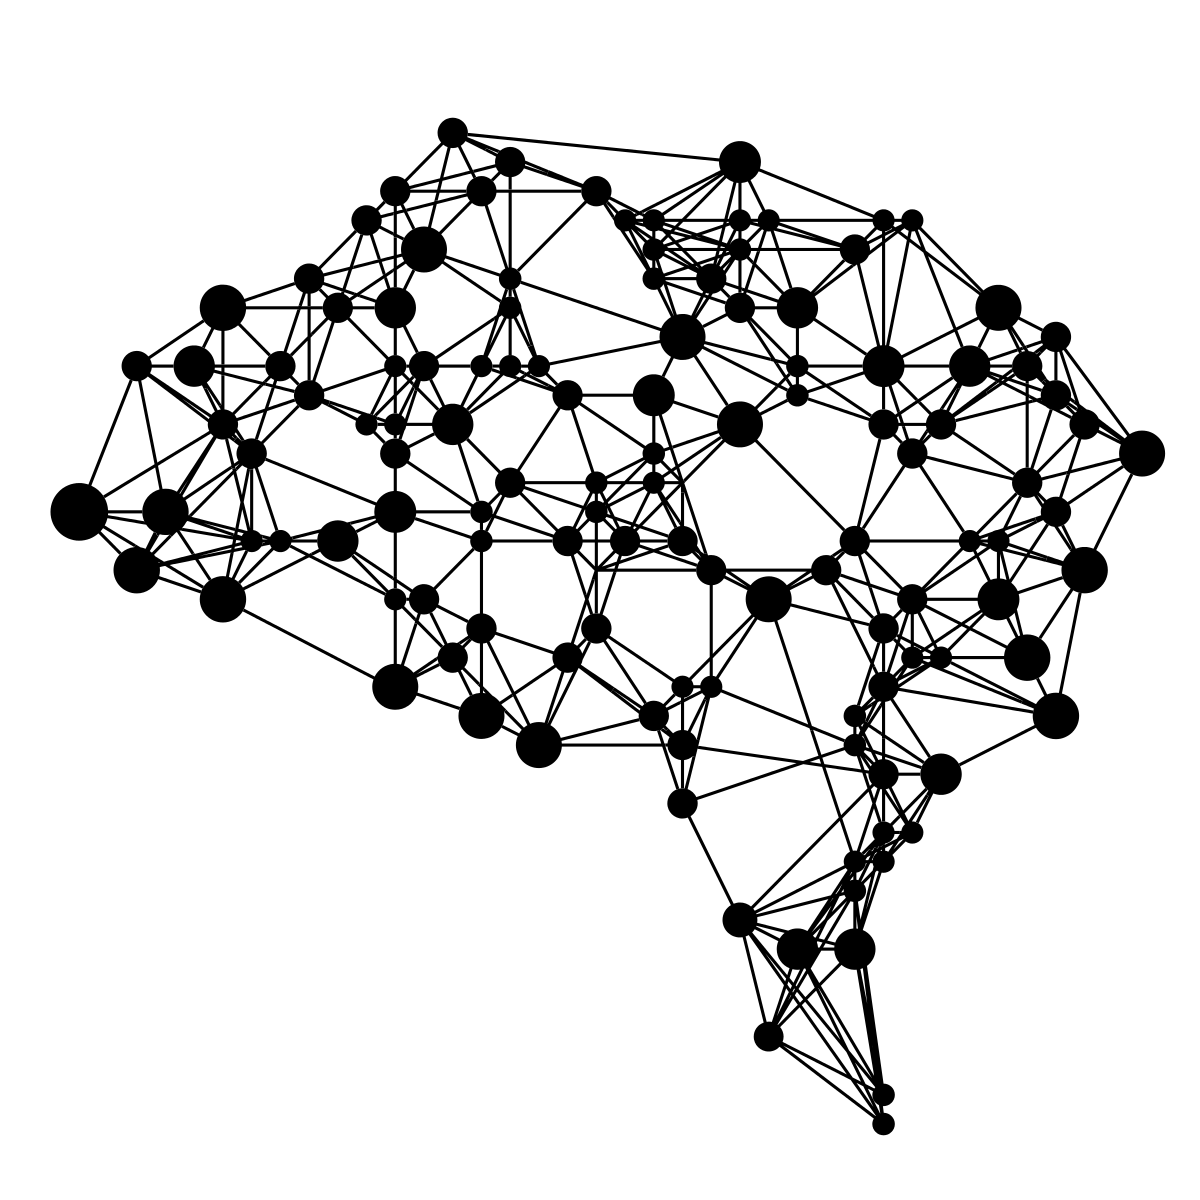
\includegraphics[totalheight=10cm]{titlepage.png}
    \cite{titlepageimage}
\end{center}

\input{lib/erklärung.tex}

\newpage
\pagenumbering{arabic}
\tableofcontents

\newpage
\input{lib/einführung.tex}%TODO: Kapitel der App einfügen

\section{Neuronale Netzwerke}

\subsection{Geschichte}

Im Jahr 1943 wurde die erste Arbeit darüber geschrieben, wie Neuronen im Gehirn funktionieren könnten und die Autoren Warren McCulloch und Walter Pitts experimentierten sogar damit diese mit elektronischen Schaltkreisen nachzubauen.\footnote[6]{\cite[]{alogicalcalculus}} In den 1950er Jahren haben Forscher von IBM daran gearbeitet ein NN\footnote[7]{Kurzform für Neuronales Netzwerk, wird ab jetzt weiterhin verwendet.} mit einem Computer zu simulieren. Der Versuch scheiterte allerdings.\footnote[8]{\cite[Absatz 3]{nnhistory}} Immer wieder gab es kleinere Forschungsprojekte, ein sehr großer Durchbruch war aber 1975 die Entwicklung eines "`Backpropagation"' Algorithmus durch den Wissenschaftler Paul Werbos. Ähnliche Algorithmen wurden wiederholt und unabhängig entwickelt, aber Werbos' Algorithmus war der erste mit großer Bedeutung.\footnote[9]{\cite[]{paulwerbosbackpropagation}} Das Prinzip des Algorithmus wird auch heute noch verwendet, es ist dieser Algorithmus der dem Neuronalen Netzwerk das selbstständige Lernen ermöglicht.\footnote[10]{siehe Kapitel \ref{funktionsweise}}
\subsubsection{Zeitstrahl}

\begin{chronology}[10]{1940}{2020}{\textwidth}
    \event{1943}{Erste Arbeit und Experimente}
    \event[1950]{1960}{Bemühungen, ein NN digital umzusetzen}
    \event{1975}{Backpropagation Algorithmus}
\end{chronology}

\subsection{Aufbau}

\begin{center}
    \begin{tikzpicture}[x=1.5cm, y=1.5cm, >=stealth]

        \foreach \m/\l [count=\y] in {1,2,3,missing,4}
        \node [every neuron/.try, neuron \m/.try] (input-\m) at (0,2.5-\y) {};

        \foreach \m [count=\y] in {1,missing,2}
        \node [every neuron/.try, neuron \m/.try ] (hidden-\m) at (2,2-\y*1.25) {};

        \foreach \m [count=\y] in {1,missing,2}
        \node [every neuron/.try, neuron \m/.try ] (output-\m) at (4,1.5-\y) {};

        \foreach \l [count=\i] in {1,2,3,n}
        \draw [<-] (input-\i) -- ++(-1,0)
        node [above, midway] {$I_\l$};

        \foreach \l [count=\i] in {1,n}
        \node [above] at (hidden-\i.north) {$H_\l$};

        \foreach \l [count=\i] in {1,n}
        \draw [->] (output-\i) -- ++(1,0)
        node [above, midway] {$O_\l$};

        \foreach \i in {1,...,4}
        \foreach \j in {1,...,2}
        \draw [->] (input-\i) -- (hidden-\j);

        \foreach \i in {1,...,2}
        \foreach \j in {1,...,2}
        \draw [->] (hidden-\i) -- (output-\j);

        \foreach \l [count=\x from 0] in {Eingabe, Versteckte, Ausgangs}
        \node [align=center, above] at (\x*2,2) {\l \\ Ebene};

    \end{tikzpicture}
\end{center}

\subsection{Funktionsweise} \label{funktionsweise}

\subsubsection{Trainieren - Backpropagation}

\section{Labelcheck als Smartphone App}\label{labelcheck}

In diesem Kapitel wird mithilfe von Python und TensorFlow ein Netzwerk erstellt und trainiert, sowie anschließend eine mobile App mit Dart und Flutter entwickelt, welche dann öffentlich für den Download bereit stehen soll.

\subsection{Die Idee}

Die Ziel ist es, dass die App es ermöglicht im Supermarkt die verschiedenen Label der Produkte zu scannen und dem Nutzer dann Auskunft über die Vertrauenswürdigkeit und generelle Aussage des Labels gibt. Die Idee habe ich in meinem Erdkunde Leistungskurs bekommen als wir über die Problematik gestoßen sind, dass die Bedeutung der verschiedenen Label eher untransparent gegenüber dem Verbraucher ist. Ich habe alle Siegel einmal im Angang \ref{angang:label} vorgestellt, da sie nur indirekt mit dem Thema der Facharbeit zusammenhängen.

\subsection{Erstellen des Models}\label{erstellen des modells}

Zum erstellen und trainieren des Modells werde ich die Sprache Python und das
Framework TensorFlow verwenden. Da sich, wie zuvor erklärt, Convolutional Neural Networks besonders gut zum Klassifiezieren von Bildern eignen werde ich im folgenden eines erstellen. 

\emph{Der vollständige Code ist im Anhang unter \ref{anhang:tfcode} einsehbar.}

\subsubsection{Trainieren des Modells mit TensorFlow und Python}

Da ich zum trainieren des Models „supervised Learning“ anwenden werde, wird ein Dataset benötigt. Dieses Dataset besteht aus vielen verschiedenen Bildern von den jeweiligen Objekten die vom Netzwerk identifiziert werden sollen. Dafür habe ich über die letzten Monate hinweg immer wieder verschiedene Label auf verschiedenen Verpackungen fotografiert und sortiert. Am Ende habe ich mich einfach darauf festgelegt die 7 Label zu benutzen, von welchen ich die meisten Fotos hatte. Supervised Learning bedeutet, dass die Daten (hier Bilder) „labelled“ sind, also das das gewünschte Ergebniss bekannt ist.41 So kann dann, zum Beispiel mit der MSE Funktion, überprüft werden wie genau das Netzwerk klassifiziert.

\subsubsection{Ergebnisse des Models}

\subsection{Entwickeln der App}

Zum entwickeln der App verwende ich die Sprache Dart und das zugehörige Framework Flutter. Im Gegensatz zu nativ geschriebenen Apps bietet Flutter die möglichkeit nur einmal den Code in Dart zu schreiben und anschließend kann die App für alle großen Platformen kompiliert werden, dazu zählen iOS, Android, aber auch Linux, Windows, MacOS und Web/Javascript. Nun muss die App ja Zugriff auf die Kamera haben und auch in die Supermärkte "`mitgebracht"' werden, weshalb nur iOS und Android relevant sind. Die App ist vollständig Quelloffen und kann auf GitHub unter \url{https://github.com/phibr0/labelcheck} eingesehen werden.

\subsubsection{Das Framework: Flutter}

Flutter Apps funktionieren anders als nativ entwickelte Apps. Herkömmliche native Apps verwenden die UI\footnote{User Interface; deutsch: Benutzeroberfläche} Komponenten des Betriebssystems und sehen daher auf jedem Gerät mit unterschiedlichen Betriebssystemversionen leicht unterschiedlich aus. Flutter hingegen stellt ein "`Canvas"' Element bereit, welches als unterliegende Grafik-Engine Google's Skia nutzt.\footnote{\cite{flutterarchitecture}; mehr dazu im Anhang \ref{anhang:flutterarc}} In Flutter stehen eine Menge UI Komponenten zur verfügung die entweder Googles Material Design guidelines oder Apples Human interface guidelines folgen. Der Dart Code stellt dann als Einzigen Eintrittspunkt die \mintinline{Dart}{main()} Methode bereit, aus welchem dann die App gestartet wird. Das Framework wird mit der Methode \mintinline{Dart}{runApp(Widget)} initialisert. In Flutter ist jedes UI Element ein "`Widget"', wodurch sich dann in Kombination in einer App große Widgethierarchien erstellen lassen. Der Code einer simplen App, welche nur den Text "`Hello World!"' in der Mitte des Bildschirms anzeigen würde, sehe demnach so aus:

\begin{wrapfigure}{l}{75mm}
  \begin{minted}[fontsize=\footnotesize,linenos]{Dart}
import 'package:flutter/widgets.dart';

void main() => runApp(MyApp());

class MyApp extends StatelessWidget {
  @override
  Widget build(BuildContext context) {
    return Center(
      child: Text('Hello World!'),
    );
  }
}
\end{minted}
\end{wrapfigure}

Zeile 1: Importieren der Widgets aus dem Framework zum bereitstellen der Klassen, wie \mintinline{Dart}{Stateless}- und \mintinline{Dart}{StatefulWidget} und den Methoden, wie \mintinline{Dart}{runApp()}.

Zeile 3: Die \mintinline{Dart}{main()} Methode mit dem einzigen Aufruf \mintinline{Dart}{runApp()}, was die Klasse \mintinline{Dart}{MyApp} als Flutter App initialisert.

Zeile 5f.: \mintinline{Dart}{MyApp} erbt die Klasse \mintinline{Dart}{StatelessWidget}, überschreibt die \mintinline{Dart}{build()} Methode und gibt eine Widgethierarchie zurück.

Zeile 8f.: Das \mintinline{Dart}{Center} Widget nimmt als einzigen benannten Parameter ein weiteres (child) Widget an, welches in diesem Fall ein \mintinline{Dart}{Text} Widget ist. Stateless bedeutet hier, dass sich der Zustand des Widgets nicht während der Laufzeit verändern kann. Im Gegensatz dazu gibt es auch noch \mintinline{Dart}{StatefulWidget}'s welche die Möglichkeit haben bei Bedarf das UI zu "`rebuilden"'.

Um der App das Aussehen von nativen Apps zu verleihen, verwendet man üblicherweise ein \mintinline{Dart}{MaterialApp} (Material Design / Android) oder \mintinline{Dart}{CupertinoApp} (Human Interface / iOS) Widget, was zudem noch wichtige Variablen, wie \mintinline{Dart}{ThemeData} für verschiedene Farben, die in der App einfach verwendet werden können oder \mintinline{Dart}{LocalizationsDelegate} welche für die Bereitstellung verschiedener Sprachen gebraucht werden, beinhaltet.

\subsubsection{Importieren des Models}

Es gibt eine speziell für mobile Geräte angepasste Version von TensorFlow mit dem Namen TensorFlow Lite. TFLite hat einen geringeren Speicherbedarf kann dafür aber auch weniger als das herkömmliche Framework.\footnote{\cite{tflite}} Implementationen dafür gibt es allerdings nicht in Dart, stattdessen verwendet man PlatformChannel's in Flutter, welche die Möglichkeit bieten platformspezifischen Code aus einer Flutter App auszuführen (Java/Kotlin für Android und Objective-C/Swift für iOS).\footnote{\cite{flutterplatformcode}}

Desweiteren muss das zuvor erstellte TensorFlow Model in ein TensorFlow Lite Model umgewandelt werden.

\subsubsection{Funktionsweise der App}

\setlength{\belowcaptionskip}{-10pt}
\begin{wrapfigure}{r}{55mm}
  \resizebox{55mm}{!}{\begin{annotatedFigure}
      {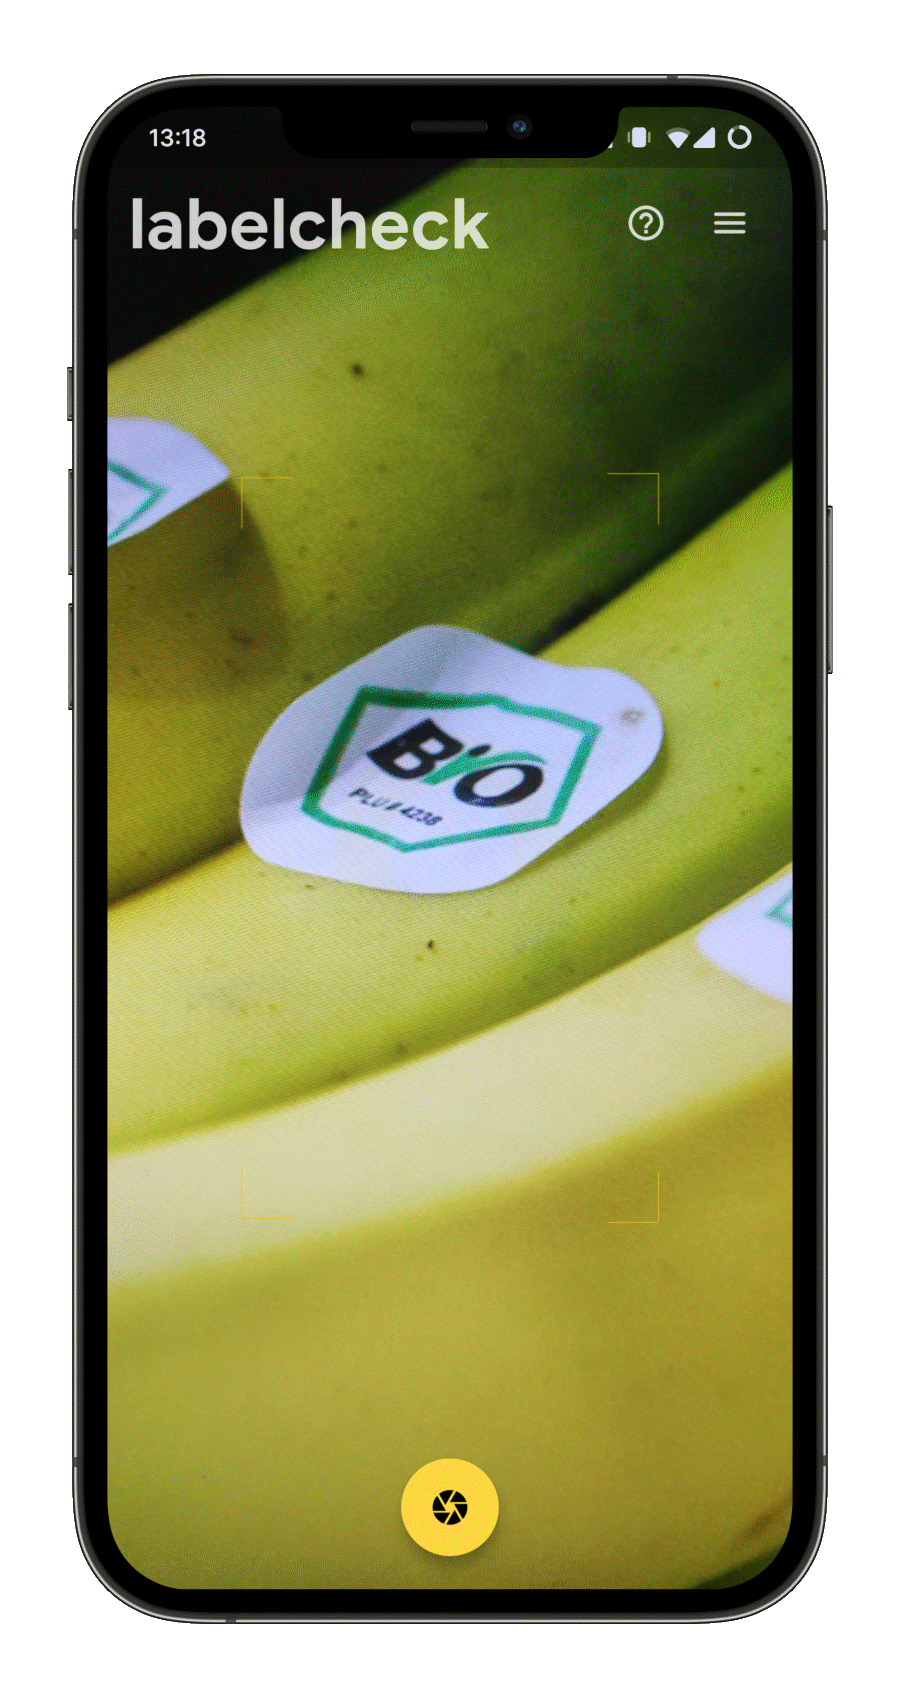
\includegraphics[width=1.0\linewidth]{labelcheckscreenshot.png}}
      \annotatedFigureBox{0.7735,0.8476}{0.8484,0.8899}{A}{0.7735,0.8476}%bl
      \annotatedFigureBox{0.2617,0.27}{0.742,0.7233}{B}{0.2617,0.27}%bl
      \annotatedFigureBox{0.432,0.076}{0.5679,0.1473}{C}{0.432,0.076}%bl
    \end{annotatedFigure}}
  \caption[]{Beispiel des Labelcheck UI's}
  \label{screenshot}
\end{wrapfigure}
\setlength{\belowcaptionskip}{0pt}

Nach dem \textbf{Start} der App werden das Model und die zugehörigen Label asynchron\footnote{hier: Im Hintergrund} geladen und anschließend TensorFlow-Lite initialisert. Der "`Floating Action Button"' \textbf{C} nimmt bei kurzem drücken ein Foto auf, speichert es temporär, schneidet es auf die Größe des "`Viewfinders'" \textbf{B} zu und ruft eine platformspezifische Methode von TensorFlow-Lite, mit dem Speicherort des Fotos als Parameter, auf. Wurde die Klassifizierung durchgeführt öffnet sich ein "`Bottom Sheet"', mit dem Namen des Labels, einer Beschreibung und einer farblichen Kennzeichnung der Wahrscheinlichkeit. Bei langem drücken von \textbf{C} passiert das gleiche, allerdings wird, anstatt des Aufnehmen eines Fotos, der Nutzer aufgefordert ein Foto aus seinen eigenen Dateien auszuwählen. Außerdem lässt sich der Knopf beliebig durch ziehen umpositionieren. Der Knopf \textbf{A} öffnet die "`Über"' Seite, auf welcher Informationen zur App, Lizenzen und Links zu dem Repository und der Datenschutzerklärung zu finden sind.

\subsubsection{Veröffentlichen der App}

Ich habe die App im Google PlayStore veröffentlicht\footnote{\url{https://play.google.com/store/apps/details?id=com.phillip.labelcheck}}, theoretisch wäre es auch möglich die App für iOS im Appstore anzubieten, leider ist ein Apple Entwicklerkonto aber mit höheren und jährlichen Kosten verbunden.

Auch musste ich eine Datenschutzerklärung bereitstellen, sie ist unter \url{https://labelcheck.phibr0.de} erreichbar.

\section{Fazit}

Ich habe in den letzen Monaten viel über die App entwicklung mit Flutter gelernt, leider habe ich mit dieser App schon etwas früher begonnen, weswegen ich heute wahrscheinlich viele Dinge anders gemacht hätte. Ich habe nicht viel darauf geachtet den UI Code von dem Logik Code zu trennen und jetzt kommt es häufig vor, dass ich lange nach etwas suchen muss. Ich plane allerdings dies noch zu beheben. Auch habe ich viele Variablen als dynamisch deklariert, was die Autovervollständigung beeinträchtigt und daher behoben werden sollte. Das beeinträchtigt allerdings nicht die Funktionalität, beziehungsweise den Nutzer sondern nur mich, solange ich noch weiter an der App arbeiten möchte. Desweiteren ist Dart in der neusten Version nun standardmäßig "`Null-Safe"'\footnote{Damit Variablen \mintinline{Dart}{null} sein können können, müssen sie speziell deklariert werden. Dies fängt viele Fehler bei Laufzeit ab.}, weswegen ich meine App auf diese Version manuell migrieren muss.

Dennoch konnte ich folgende Funktionen erfolgreich implementieren:

\begin{itemize}
  \item Übersetzungen für Englisch und Deutsch, sowie automatischem Anpassen an die Systemsprache
  \item Modernes Design nach Material Design Guidelines
        \begin{itemize}
          \item Automatischer Wechsel zwischen hellem und dunklem Modus
        \end{itemize}
  \item Automatisches Sammeln von anonymisierten Nutzerstatistiken und Absturzberichten durch Google Analytics/Firebase Crashlytics
        \begin{itemize}
          \item Zusätzlich manuelle Fehlerberichterstattung durch den Nutzer via E-Mail
        \end{itemize}
  \item Integration der Wikipedia API für noch mehr Informationen über das Label
  \item Klassifizieren von Fotos, entweder in der App aufgenommen oder aus einer Datei
  \item Hosten einer Website für die Datenschutzerklärung und Nutzungsbedingungen
\end{itemize}

Auch habe ich einen größeren Einblick in die unterliegende Mathematik von Neuronalen Netzen erhalten. Alles in einem würde ich sagen die Facharbeit war für mich ein Erfolg.

\newpage
\appendix
\label{Anhang}
\section{Anhang}

\subsection{Weitere Aktivierungsfunktionen}\label{anhang:weitereaktivierungsfunktionen}

\begin{figure}[h]
    \center
    \begin{tikzpicture}
    \begin{axis}
        [
            grid=major,
            xmin=-3,
            xmax=3,
            axis x line=bottom,
            ytick={0,1,2},
            ymax=2.5,
            ymin=-0.5,
            axis y line=middle,
            legend style={at={(0.5,-0.2)},anchor=north}
        ]
        \addplot[red,mark=none]{(x>=0)*x};
        \addplot[blue, mark=none]{0.5*(tanh(\x)+1)};
        \legend{ReLU - $\max{(0,x)}$, (Verschobene) Hyperbolische Tangente - $0.5(\tanh{(x)}+1)$}
    \end{axis}
\end{tikzpicture}
    \caption[Aktivierungsfunktionen]{Weitere Aktivierungsfunktionen, ergänzend zu der Sigmoid Funktion aus Kapitel \ref{funktionsweise}}
    \label{Aktivierungsfunktionen}%
\end{figure}

Die ReLU (Rectified linear Unit) Funktion ist im Vergleich zu anderen Aktivierungsfunktionen, wie der Sigmoidfunktion oder der Hyperbolischen Tangente, deutlich simpler, was sich in Leistungsansprüchen des Trainingsprozesses wiederspiegelt.\footnote{\cite{nnfs}}

\subsection{Code für das Beispiel aus \ref{funktionsweise}}\label{anhang:colab1}

\begin{listing}[H]
    \begin{minted}[fontsize=\footnotesize,linenos]{python}
import tensorflow as tf
import tensorflow.keras.layers as layers

numberOfNeuronsInFirstLayer = 16 
numberOfNeuronsInSecondLayer = 16 
numOfEpochs = 5 

mnist = tf.keras.datasets.mnist

(x_train, y_train), (x_test, y_test) = mnist.load_data() # Laden des MNIST Datasets
# Und aufteilen in Trainigsdaten und Testdaten

x_train = tf.keras.utils.normalize(x_train, axis=1) # Normalisieren des Datasets
x_test = tf.keras.utils.normalize(x_test, axis=1)

model = tf.keras.models.Sequential() # Erstellen des Neuronalen Netzwerks
model.add(layers.Flatten())
model.add(layers.Dense(numberOfNeuronsInFirstLayer, activation=tf.nn.sigmoid))
# Hinzufügen der Layer
model.add(layers.Dense(numberOfNeuronsInSecondLayer, activation=tf.nn.sigmoid))
model.add(layers.Dense(10, activation=tf.nn.softmax))

model.compile(optimizer='adam',
              loss='sparse_categorical_crossentropy',
              metrics=['accuracy']) # Kompilieren der Layer zu einem trainierfähigen Modell

model.fit(x_train, y_train, epochs=numOfEpochs)
# Trainieren des Modells mit den Trainingsdaten und x Epochen

model.save('beispielModel_MNIST') # Speichern des Modells

    \end{minted}
    \caption{Umsetzung mit Python und Tensorflow}
\end{listing}
Ein interaktives Beispiel gibt es zusätzlich hier in meinem Colab Notebook: \url{https://bit.ly/34Ggfuh}\footnote{Ungekürzter Link: \url{https://colab.research.google.com/drive/1ty_QQlL038YT6KpBjSdqGvIGyH0YXwxW}}

\subsection{Labelcheck Code}\label{anhang:labelchecktf}

asdf

\subsection{Die Flutter Architektur}\label{anhang:flutterarc}

\begin{figure}[H]
    \centering
    \resizebox{\textwidth}{!}{
    \includesvg{assets/flutterarchitecture}
    }
    \caption{Flutter's Architektur (\cite{flutterarchitecture})}
\end{figure}

Flutters Architektur ist in drei Ebenen unterteilt. Als Basis die "`Embedder Ebene"', welche für jede Platform angepasst werden muss und zum Beispiel für das Thread Management zuständig ist. Dadrüber liegt die "`Engine Ebene"', welche zu einem Großteil in C++ geschrieben ist und zu welcher auch die Grafikengine Skia gehört. Dadrüber liegt die "`Framework Ebene"', welche zum Beispiel die UI Komponenten beinhaltet und komplett in Dart entwickelt wird.\footnote{\cite{flutterarchitecture}}

\newpage
\printbibliography[heading=bibintoc, title={Literaturverzeichnis}]

\end{document}